%%% Lecture 1 Slides %%%

\documentclass{beamer}

%\documentclass[handout]{beamer}
%\usepackage{pgfpages}
%\pgfpagesuselayout{2 on 1}[a4paper,border shrink=5mm]
%\pgfpagesuselayout{1 on 1}[a4paper,border shrink=5mm]



\usepackage{amssymb}
\usepackage{amsmath}
\usepackage{mathtools}
\usepackage{tikz}
\usetikzlibrary{shapes,arrows}
\usetikzlibrary{positioning}
\usetikzlibrary{trees}
\usepackage{pgfplots}
\usepackage{pdflscape}
\usepackage{graphicx}
\usepackage{colortbl}
\usepackage{listings}
\usepackage{adjustbox}

\DeclarePairedDelimiter{\ceil}{\lceil}{\rceil}

\newcommand{\bs}{\boldsymbol}
\newcommand{\mb}{\mathbf}
\newcommand{\indep}{{\bot\negthickspace\negthickspace\bot}}
\newcommand{\notindep}{{\bot\negthickspace\negthickspace\bot}{\negthinspace
  \negmedspace \negthickspace \negthickspace \diagup
  \;}}
\renewcommand{\S}{\mb{S}}
\usepackage{color}
\definecolor{direct}{HTML}{FF0000}
\definecolor{indirect}{HTML}{FF9999}
\definecolor{dirin}{HTML}{990000}
\definecolor{control}{HTML}{999999}
\definecolor{directE}{HTML}{ED1C24}
\definecolor{indirectE}{HTML}{F69679}
\definecolor{controlE}{HTML}{999999}

%\defV{{\rm Var}\,}
\def\E{{\rm E}\,}
\def\arg{{\rm arg}\,}
\def\Cov{{\rm Cov}\,}
\def\N{{\rm N}\,}
\newcommand{\plim}{{\rm plim} \,}
\DeclareMathOperator*{\argmin}{arg\,min}
\newcommand{\X}{\mathbf{X}}
\newcommand{\Y}{\mathbf{Y}}
\newcommand{\Z}{\mathbf{Z}}
\newcommand{\I}{\mathbf{I}}
\newcommand{\V}{\mathbf{\Omega}}
\newcommand{\W}{\mathbf{W}}
\newcommand{\R}{\mathbf{R}}
\newcommand{\A}{\mathbf{A}}
\newcommand{\B}{\mathbf{B}}
\newcommand{\D}{\mathbf{D}}
\newcommand{\T}{\mathbf{T}}
\newcommand{\F}{\mathbf{F}}
\renewcommand{\O}{\mathbf{O}}
\renewcommand{\H}{\mathbf{H}}
\newcommand{\g}{\mathbf{g}}
\renewcommand{\r}{\mathbf{r}}
\newcommand{\s}{\mathbf{s}}
\newcommand{\uu}{\mathbf{u}}
\newcommand{\w}{\mathbf{w}}
\newcommand{\x}{\mathbf{x}}
\newcommand{\vv}{\mathbf{v}}
\newcommand{\z}{\mathbf{z}}
\newcommand{\y}{\mathbf{y}}

\newcommand{\bi}{\begin{itemize}}
\newcommand{\ei}{\end{itemize}}
\newcommand{\be}{\begin{enumerate}}
\newcommand{\ee}{\end{enumerate}}

\newcommand{\Beta}{\boldsymbol{\beta}}
\newcommand{\btheta}{\boldsymbol{\theta}}
\newcommand{\bgamma}{\boldsymbol{\gamma}}
\newcommand{\bpi}{\boldsymbol{\pi}}
\newcommand{\arrowp}{\stackrel{p}{\rightarrow}}
\newcommand{\arrowd}{\stackrel{d}{\rightarrow}}
\newcommand{\0}{\mathbf{0}}
\newcommand{\bP}{\mathbf{P}}
\newcommand{\nn}{\nonumber}
\def\S{{\sigma}}
\def\Supp{{\rm Supp}\,}


\newcommand\independent{\protect\mathpalette{\protect\independenT}{\perp}}
\def\independenT#1#2{\mathrel{\rlap{$#1#2$}\mkern2mu{#1#2}}}

\newcommand{\vsf}{\vspace{.5cm}}

\usepackage[english]{babel}
% or whatever

\usepackage[latin1]{inputenc}
% or whatever

\usepackage{times}
\usepackage[T1]{fontenc}
\setbeamertemplate{footline}[page number]{}
\setbeamertemplate{navigation symbols}{}


\title[Lecture 2: Population Inference for Proportions] % (optional, use only with long paper titles)
{Lecture 2: Population Inference for Proportions}


\begin{document}

\begin{frame}
  \titlepage
\end{frame}


\frame{
\frametitle{Review}

\begin{itemize}
\item Last lecture, we discussed description/summarization with means, conditional means, and differences in conditional means.
\item We considered the properties of these summaries (e.g., balance point, least squares, etc.) and how much was left out by summarizing (e.g., squared residuals)
\item This was done in the context where we only cared about the sample, either provisionally or because we had sampled everyone (i.e., a census).
\end{itemize}

}
\frame{
\frametitle{Today}

\begin{itemize}
\item Today we consider the context where we have a random sample from a large population and we have measured a binary outcome. 
\item Our goal over the next couple of lectures is to summarize the population with population means, conditional population means, and differences in conditional population means.
\item Summarizing data we don't have (everything in the population that isn't in the sample) is more difficult than summarizing data we do have (sample).
\end{itemize}

}

%\frame{
%\frametitle{Outline}
%
%\begin{itemize}
%\item Population Inference for proportions
%\item Population Inference for means
%\end{itemize}
%
%}

\frame{
\frametitle{Sample}


Suppose that a week before the 2020 presidential election, you contacted a sample of $n=625$ potential Georgia voters, randomly selected (with replacement) from the population of  $N = 7,233,584$ on the public voters register, to ask whether they planned to vote.\\
\pause
\vspace{.3cm}


Suppose also that all potential voters can be contacted, will respond honestly to your questions, and will not change their minds about voting.
\pause

\begin{table}[h]
\begin{center}
\caption{Sample}\label{t:sam}
\begin{tabular}{r|rrrrrr|r}
$i$ & 1 & 2 & 3 & 4 & $\dots$ & 625 & $\bar{y}_{625}$  \\
$y_i$ & 1 & 1 & 0 & 1 & $\dots$ & 0 & .66 \\
\end{tabular}
\end{center}
\end{table}
\pause
Remember that the mean of a binary variable is a proportion.
}

\frame{
\frametitle{Sample versus Population}

\begin{table}[h]
\begin{center}
\caption{Sample}\label{t:sam}
\begin{tabular}{r|rrrrrr|r}
$i$ & 1 & 2 & 3 & 4 & $\dots$ & 625 & $\bar{y}_{625}$  \\
$y_i$ & 1 & 1 & 0 & 1 & $\dots$ & 0 & .68 \\
\end{tabular}
\end{center}
\end{table} \pause

After election day, we found that in fact $4,999,960$ people, or roughly 70\% of registered voters, turned out to vote.
\begin{table}[h]
\begin{center}
\caption{Population}\label{t:pop}
\begin{tabular}{r|rrrrrrrrr|r}
$j$ & 1 & 2 & 3 & 4 & $\dots$ & $\dots$     & $\dots$& $\dots$ & 7,233,584 & $\bar{y}_{7,233,584}$  \\
$y_j$ & 0 & 1 & 0 & 1 & $\dots$& $\dots$  & $\dots$& $\dots$ & 1 & .70  \\
\end{tabular}
\end{center}
\end{table}


}

\frame{
\frametitle{Two Questions}

\begin{enumerate}
\item .68 is close to .70, did we get lucky?
\item Could we have predicted how close we would get before seeing the .70? 
\end{enumerate}

}

\frame{
\frametitle{Sampling Distribution of $\overline{Y}_{625}$}

\begin{table}[h]
\begin{center}
%\caption{Sampling Distribution of $\overline{Y}_{625}$}\label{t:samdist}
{\footnotesize
\begin{tabular}{r|rr|rr|r|rr|r}
$i$ & \multicolumn{2}{r|}{1} & \multicolumn{2}{r|}{2}   & $\dots$ & \multicolumn{2}{r|}{625} &    \\
\visible<2->{$s$} & $J_1$ & $Y_1$ & $J_2$ & $Y_2$   & $\dots$ & $J_{625}$ & $Y_{625}$  & $\overline{Y}_{625}$  \\
\hline
\visible<2->{1}  &  9562350& 1& 8763351 & 1   & $\dots$ &  1294801 & 0 & .68 \\
\visible<2->{2} &  \visible<2->{5331704}& \visible<2->{0}& \visible<2->{4533839} & \visible<2->{1}   & \visible<2->{$\dots$} & \visible<2->{3342359} & \visible<2->{1} & \visible<2->{.70} \\
\visible<3->{3} & \visible<3->{5129936}& \visible<3->{0}& \visible<3->{10981600} & \visible<3->{0}  & \visible<3->{$\dots$} & \visible<3->{4096184} & \visible<3->{1} & \visible<3->{.75} \\
\visible<3->{4} &  \visible<3->{803605}& \visible<3->{0}& \visible<3->{7036389} & \visible<3->{1} & \visible<3->{$\dots$} & \visible<3->{803605} & \visible<3->{0} & \visible<3->{.73} \\
\visible<3->{5} &  \visible<3->{148567} & \visible<3->{0}& \visible<3->{3833847} & \visible<3->{1}  & \visible<3->{$\dots$} & \visible<3->{4769869} & \visible<3->{1} & \visible<3->{.69} \\
\visible<3->{$\vdots$} & \visible<3->{$\vdots$} & \visible<3->{$\vdots$}  & \visible<3->{$\vdots$} & \visible<3->{$\vdots$}  & \visible<3->{$\vdots$} & \visible<3->{$\vdots$} & \visible<3->{$\vdots$} &  \visible<3->{$\vdots$} \\ 
\visible<3->{1 mil} &  \visible<3->{4163458} & \visible<3->{0}& \visible<3->{8384613} & \visible<3->{1}& \visible<3->{$\dots$} & \visible<3->{377981} & \visible<3->{1} & \visible<3->{.74} \\
 \visible<3->{$\vdots$} & \visible<3->{$\vdots$} & \visible<3->{$\vdots$} & \visible<3->{$\vdots$} & \visible<3->{$\vdots$}  & \visible<3->{$\vdots$} & \visible<3->{$\vdots$} & \visible<3->{$\vdots$}  & \visible<3->{$\vdots$} \\ 
\hline
\visible<4->{$f_{\cdot}(\cdot)$} & \multicolumn{2}{r|}{\visible<5->{Bern(.70)}} & \multicolumn{2}{r|}{\visible<5->{Bern(.70)}}  & & \multicolumn{2}{r|}{\visible<5->{Bern(.70)}} & \visible<6->{$\frac{Bin(625,.70)}{625}$} \\
\end{tabular}}
\end{center}
\end{table} 

\begin{itemize}
\item<4-> What is the distribution of $Y_1$?
\item<5-> What is the distribution of $\sum_{i}^{625}Y_i$?
\item<6-> What two numbers show that we sampled with replacement?
\end{itemize}
}

\frame{
\frametitle{Review of Bernoulli and Binomial Distributions}


We can write distributions for our random variables (RVs) that describe the probability of getting particular values for these variables.\\
\pause
\vspace{.3cm}

$Y_1,...,Y_{625}$ are Bernoulli RVs:
\begin{align*}
f_{Y_1}(y_1) &= (.71)^{y_1} (.29)^{1-y_1} \text{ for } y_1=0,1\\
\vdots \quad  &=   \quad\quad\quad\quad\quad\quad \vdots  \\
f_{Y_{625}}(y_{625}) &= (.71)^{y_{625}} (.29)^{1-y_{625}} \text{ for } y_{625}=0,1
\end{align*} 
\pause

$\sum_{i=1}^{625} Y_i$ is a Binomial RV:
\small
\begin{align*}
f_{\sum_{i=1}^{625} Y_i}(\sum_{i=1}^{625} y_i) = {625 \choose k} (.70)^{\sum_{i=1}^{625} y_i} (.30)^{625-\sum_{i=1}^{625} y_i} \text{ for } \sum_{i=1}^{625} y_i=0,\dots,625
\end{align*} 

}

\begin{frame}[fragile]
\frametitle{The Sampling Distribution in \texttt{R}}

\begin{verbatim}
# Resample the number of voters 1,000,000 
# times and store these 1,000,000 
# numbers in a vector.
\end{verbatim} \pause
\begin{verbatim}
sumY_vec <- rbinom(1000000, size=625, prob=.70) 
\end{verbatim} \pause
\begin{verbatim}
# Divide all of these numbers 
# by the sample size.

Ybar_vec <- sumY_vec/625
\end{verbatim} \pause
\begin{verbatim}
# Plot a histogram

hist(Ybar_vec)
\end{verbatim} 

\end{frame}

\frame{

\begin{figure}[ht] \centering
        \scalebox{.5}{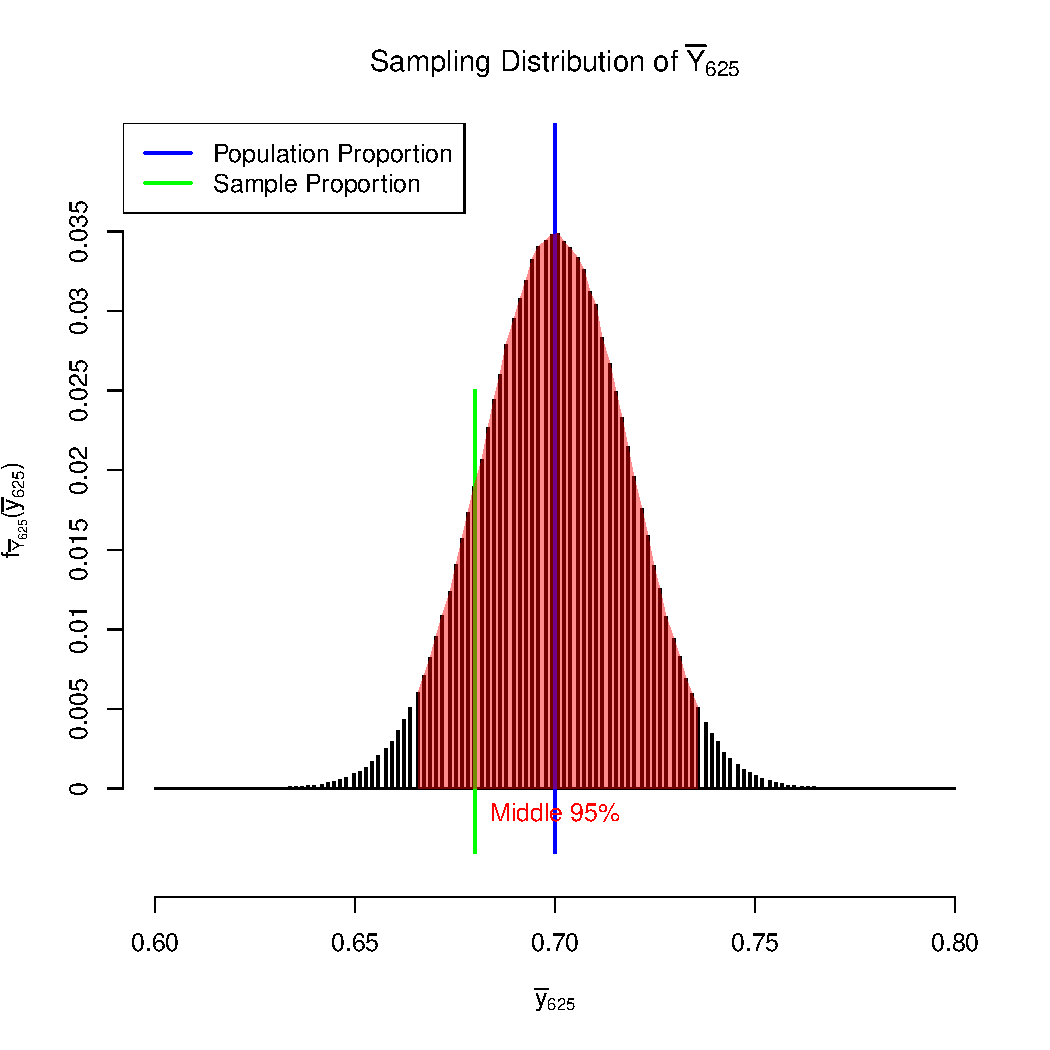
\includegraphics{figs/samdist.pdf}}
\end{figure}

}

\frame{
\frametitle{Two Questions}

\begin{enumerate}
\item .68 is close to .70, did we get lucky? \pause No! In a million runs, almost all within .05.\pause
\item Could we have predicted how close we would get before seeing the .70?
\end{enumerate}

}

\frame{
\frametitle{Predicting before election day}

Could we have predicted how close we would get? \pause Yes, in a sense.\pause
\begin{itemize}
\item We will use a confidence interval. \pause
\item A confidence interval has a width, which answers the ``how close'' question. \pause
\item However, a confidence interval also has a coverage probability. \pause This probability will almost never be 100\%.
\end{itemize}

}

\frame{
\frametitle{CI Coverage of $\overline{Y}_{625} \pm .01$}

As an exercise, let's arbitrarily choose a width of 2\% and use the sampling distribution.

\begin{table}[h]
\begin{center}
%\caption{Sampling Distribution of $\overline{Y}_{625}$}\label{t:samdist}
{\footnotesize
\begin{tabular}{r|r|r|r|r|r|r}
$i$ & \multicolumn{1}{r|}{1} & \multicolumn{1}{r|}{2}   & $\dots$ & \multicolumn{1}{r|}{625} &  &  \\
\visible<2->{$s$} & $Y_1$  & $Y_2$   & $\dots$  & $Y_{625}$  & $\overline{Y}_{625}$ &  $\overline{Y}_{625} \pm .01$\\
\hline
\visible<2->{1}  & 1 & 1   & $\dots$  & 0 & .68 & [.67,.69] \\
\visible<2->{2} & \visible<2->{0} & \visible<2->{1}   & \visible<2->{$\dots$}  & \visible<2->{1} & \visible<2->{.70} & \visible<2->{[.69,.71]} \\
\visible<3->{3} & \visible<3->{0}& \visible<3->{0}  & \visible<3->{$\dots$} & \visible<3->{1} & \visible<3->{.75} & \visible<3->{[.74,.76]} \\
\visible<3->{4} &  \visible<3->{0}& \visible<3->{1} & \visible<3->{$\dots$}  & \visible<3->{0} & \visible<3->{.73} & \visible<3->{[.72,.74]} \\
\visible<3->{5}  & \visible<3->{0} & \visible<3->{1}  & \visible<3->{$\dots$}  & \visible<3->{1} & \visible<3->{.69} & \visible<3->{[.68,.70]} \\
\visible<3->{$\vdots$}  & \visible<3->{$\vdots$} & \visible<3->{$\vdots$}   & \visible<3->{$\vdots$} & \visible<3->{$\vdots$} &  \visible<3->{$\vdots$}&  \visible<3->{$\vdots$} \\ 
\visible<3->{1 mil} & \visible<3->{0} & \visible<3->{1}& \visible<3->{$\dots$}  & \visible<3->{1} & \visible<3->{.74} & \visible<3->{[.73,.75]} \\
 \visible<3->{$\vdots$}   & \visible<3->{$\vdots$} & \visible<3->{$\vdots$}  & \visible<3->{$\vdots$} & \visible<3->{$\vdots$}  & \visible<3->{$\vdots$} & \visible<3->{$\vdots$} \\ 
\hline
%\visible<4->{$f_{\cdot}(\cdot)$} & \multicolumn{1}{r|}{\visible<5->{Bern(.70)}} & \multicolumn{1}{r|}{\visible<5->{Bern(.70)}}  & & \multicolumn{1}{r|}{\visible<5->{Bern(.70)}} & \visible<6->{$\frac{Bin(625,.70)}{625}$} \\
\end{tabular}}
\end{center}
\end{table} 

}

\begin{frame}[fragile]
\frametitle{Coverage of $\overline{Y}_{625} \pm .01$ in \texttt{R}}

\begin{verbatim}
# Resample the number of voters 1,000,000 
# times and store these 1,000,000 
# numbers in a vector.
\end{verbatim} \pause
\begin{verbatim}
sumY_vec <- rbinom(1000000, size=625, prob=.70) 
\end{verbatim} \pause
\begin{verbatim}
# Divide all of these numbers 
# by the sample size.

Ybar_vec <- sumY_vec/625
\end{verbatim} \pause
\begin{verbatim}
# Calculate coverage

mean(Ybar_vec-.01 <= .7 & Ybar_vec+.01 >= .7 ) 
# about 40\%
\end{verbatim} 

\end{frame}

\frame{
\frametitle{Calibrating the CI}

The previous exercise doesn't address our question because
\begin{enumerate}
\item We won't have access to the sampling distribution before election day.
\item We don't want to choose the width and receive the coverage, we want to choose coverage and receive the width
\end{enumerate} 

There are many ways to calibrate a CI (choose a coverage, receive the width) without observing the sampling distribution. We will explore the percentile bootstrapping approach for getting a CI with 95\% coverage for the remainder of this lecture. 

  

}


\begin{frame}[fragile]
\frametitle{Bootstrapped Sampling Distributions}

At the time of our sample, we don't observe the population or population proportion (.70), so we cannot construct the sampling distribution.\\
\pause
\vspace{.5cm}

However, we can take repeated random samples \emph{with replacement} of size 625 from the sample of size 625.

\begin{table}[h]
\begin{center}
\caption{Sample}\label{t:sam}
\begin{tabular}{r|rrrrrr|r}
$i$ & 1 & 2 & 3 & 4 & $\dots$ & 625 & $\bar{y}_{625}$  \\
$y_i$ & 1 & 1 & 0 & 1 & $\dots$ & 0 & .68 \\
\end{tabular}
\end{center}
\end{table}
\pause

The is equivalent to replacing .70 with .68 in the \texttt{R} code.
\begin{verbatim}
sumY_vec <- rbinom(1000000, size=625, prob=.68) 
\end{verbatim} 


\end{frame}


\frame{
\begin{figure}[ht] \centering
        \scalebox{.5}{
\includegraphics{figs/estsamdist.pdf}}
\end{figure}

}


\frame{
\frametitle{The Logic of Confidence Intervals}

If the bootstrapped sampling distribution has the same shape as the sampling distribution,
\begin{enumerate}
\item The 95\% confidence interval will \emph{cover} the population proportion when the sample proportion is in the middle 95\% of the sampling distribution. \pause

\item The 95\% confidence interval will \emph{not} cover the population proportion when the sample proportion is not in the middle 95\% of the sampling distribution. \pause

\item There is a 95\% probability of getting a sample proportion in the middle 95\% of the sampling distribution, therefore there is 95\% probability of getting a 95\% confidence interval that covers the population proportion. 
\end{enumerate}
}




\frame{
\begin{figure}[ht] \centering
        \scalebox{.5}{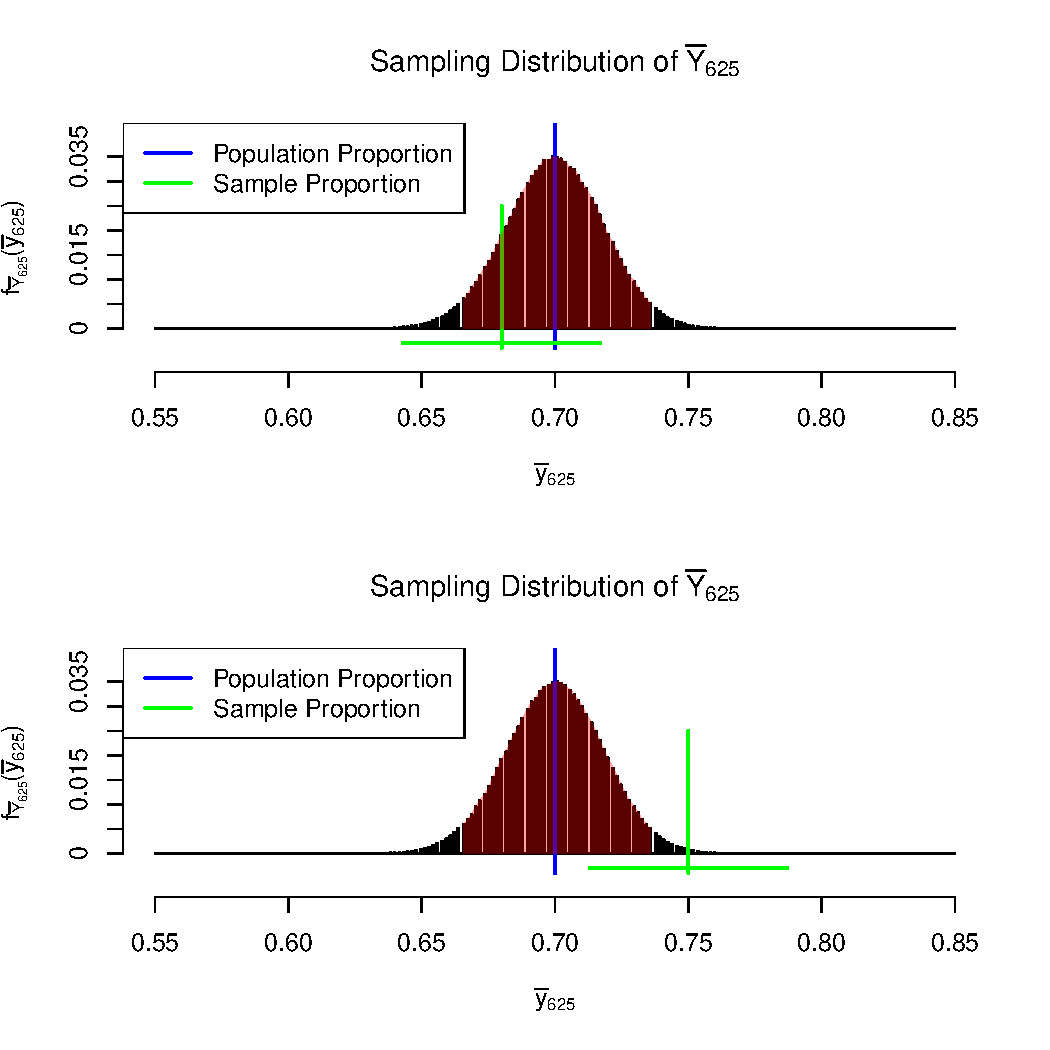
\includegraphics{figs/samdistCI.pdf}}
\end{figure}

}

\frame{
\frametitle{The Sampling Distribution of the Confidence Interval}
\begin{table}[h]
\begin{center}
{\footnotesize
\begin{tabular}{r|r|r|r|r|rc}
$i$ & \multicolumn{1}{r|}{1} & \multicolumn{1}{r|}{2}   & $\dots$ & \multicolumn{1}{r|}{625} & &   \\
$s$  & $Y_1$  & $Y_2$   & $\dots$  & $Y_{625}$  & $\overline{Y}_{625}$ & \multicolumn{1}{c}{95\% CI} \\
\hline
1 & 1 & 1   & $\dots$  & 0 & .68  & \visible<2->{[.643,.717]}\\
2 & 0 & 0  & $\dots$  & 1 & .75  & \visible<3->{[.715,.785]}\\
3 & 0 & 1   & $\dots$  & 1 & .70  & \visible<4->{[.663,.737]}\\
4 & 0 & 1 & $\dots$  & 1 & .73  & \visible<4->{[.694,.766]}\\
5 & 0 & 1  & $\dots$  & 1 & .69 & \visible<4->{[.653,.727]}\\
$\vdots$ & $\vdots$  & $\vdots$ & $\vdots$ & $\vdots$  & $\vdots$ & \visible<4->{$\vdots$}  \\ 
1 mil  & 0 & 1& $\dots$  & 1 & .74 & \visible<4->{[.705,.775]}\\
 $\vdots$  & $\vdots$  & $\vdots$ & $\vdots$ & $\vdots$  & $\vdots$  & \visible<4->{$\vdots$}\\ 
\hline
\end{tabular}}
\caption{\emph{Sampling Distributions for $\overline{Y}_{625}$ and the 95\% Confidence Interval}}\label{t:samdistCI}
\end{center}
\end{table}

95\% of the rows in this sampling distribution will have a CI that covers .70.

}


\frame{
\frametitle{Why do the distributions have the same shape?}

Informal logic:
\begin{enumerate}
\item If $n$ is big enough, the sampling distribution of the proportion is approximately normally distributed due to the De Moivre - Laplace Theorem. \pause
\item We can observe that the bootstrapped sampling distribution of the proportion is approximately normally distributed.\pause
\item The variance fully characterizes the shape of a normal distribution (not the location). \pause
\item The variance of the sampling distribution of the proportion is $\sqrt{.7 (1-.7)/625}=.0183$.\pause
\item The variance of the bootstrapped sampling distribution of the proportion is $\sqrt{.68 (1-.68)/625}=.0187$.\pause
\item When $n$ is large, these variances are close. 
\end{enumerate}

}

\frame{
\frametitle{Two Questions}

\begin{enumerate}
\item .68 is close to .70, did we get lucky?  No! In a million runs, almost all within .05.
\item Could we have predicted how close we would get before seeing the .70? \pause Yes! \pause Confidence intervals.
\end{enumerate}

}

\frame{
\frametitle{Summary of Population Inference for Proportions}

\begin{itemize}
\item
\end{itemize}


}





\end{document}

